\section{Collimator\_radial: A radial Soller blade collimator}

\component{Collimator\_radial}{System, E.Farhi}{$w_1$, $h_1$, $w_2$, $h_2$, $len$, $\theta_{min}$, $\theta_{max}$, $nchan$, $radius$, $divergence$ (in deg.)}{$nblades$, $roc$ and others}{validated, position is center of radius}

\begin{figure}
  \begin{center}
    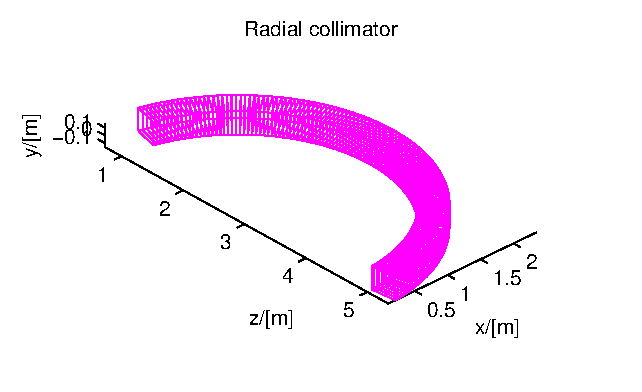
\includegraphics[width=0.9\textwidth]{figures/radial.eps}
  \end{center}
\caption{A radial collimator}
\label{f:coll-radial}
\end{figure}

This is a radial collimator that works either using the same approximation as the Collimator\_linear (see section \ref{collimator-linear}), or with an exact model but a lower statistics.

The geometry description requires to define the inner radius $radius$, the radial length $len$, the input and output window dimensions $w_1$, $h_1$, $w_2$, $h_2$, the number of Soller channels $nchan$ (each of then being a single linear collimator) arranged with the [$\theta_{min}$, $\theta_{max}$] angle with respect to the Z-axis.

If the $divergence$ parameter is defined, then the approximation level is used as in the Collimator\_linear component (see section \ref{collimator-linear}). On the other hand, if you perfer to describe exactly the number of blades $nblades$ assembled to build a single collimator channel, then the model is exact, and traces the neutron trajectory inside each Soller. The computing efficiency is then lowered by a factor 2.

The component can be made oscillating with an amplitude of $roc$ times $\pm w_1$.
